\documentclass[11pt,twocolumn,notitlepage,openany,twoside]{book}
\usepackage[paperheight=11.25in,paperwidth=8.75in, margin=0.625in]{geometry}
\usepackage{titlesec}
\usepackage{verbatim}
\pagestyle{headings}

% Figure setup
\usepackage[]{graphicx}
\graphicspath{ {figures/} }
\usepackage{float}
\setlength{\floatsep}{0pt plus 2.0pt minus 2.0pt}
\setlength{\dbltextfloatsep}{5pt plus 2.0pt minus 2.0pt}
\usepackage{caption}

% % Table setup
% \usepackage[table]{xcolor}
% \usepackage{array}
% \newcolumntype{L}[1]{>{\raggedright\let\newline\\\arraybackslash\hspace{0pt}}m{#1}}
% \usepackage{multirow}
%
% \newcommand*{\tabbox}[2][t]{%
%     \vspace{0pt}\parbox[#1][1.7\baselineskip]{8pt}{\strut#2\strut}}
%
% \newcommand*{\tabboxb}[2][t]{%
%     \vspace{0pt}\parbox[#1][2.2\baselineskip]{8pt}{\strut#2\strut}}

% Remove the giant space at the beginning of a chapter
\titleformat{\chapter}[display]
    {\normalfont\huge\bfseries}{\chaptertitlename\ \thechapter}{20pt}{\Huge}
\titlespacing*{\chapter}{0pt}{0pt}{20pt}

\title{Metabolic interactions and capabilities within microbial communities}
\author{Gregory Leonard Medlock}


% % Optimization problem formatting
% \usepackage{amsmath}
%
% % Bibliography setup
% \usepackage[backend=biber, style=numeric-comp,sorting=none,terseinits=true, giveninits=true,maxbibnames=4]{biblatex}
% \addbibresource{rf_references.bib}
% \DeclareNameAlias{default}{last-first}
% \renewcommand*{\revsdnamepunct}{}
% \renewcommand*{\bibfont}{\small}

\begin{document}
\frontmatter

\begingroup
\let\clearpage

\tableofcontents
\hspace{1.5cm}
\listoffigures
\hspace{1.5cm}
\listoftables

\endgroup

\clearpage
\addcontentsline{toc}{chapter}{Acknowledgments}
\section*{Acknowledgments}

Acknowledgements will be here

\mainmatter


%------------------------------------------------------------------------------------
% Chapter 1 Introduction
%------------------------------------------------------------------------------------
\chapter{Introduction}
%\begin{refsection}

\section{Specific Aims}

These the aims:

\begin{enumerate}
  \item \textbf{Aim 1: Identify \textit{in vitro} metabolic interactions between members of a defined mouse microbiota}. Aim 1
  \item \textbf{Aim 2: Develop an ensemble-driven framework for the refinement and application of genome-scale metabolic network reconstructions of gut microbes}. Aim 2
\end{enumerate}



\section{A Preview of this Dissertation}

Preview text

%\end{refsection}

%------------------------------------------------------------------------------------
% Chapter 2
%------------------------------------------------------------------------------------
\chapter{Inferring Metabolic Mechanisms of Interactions within a Defined Gut Microbiota}
\chaptermark{Metabolic interactions}

%\begin{refsection}

The contents of this chapter are published as a research article here:

\medskip\noindent
Medlock GL, MA Carey, DG McDuffie, MB Mundy, N Giallourou, JR Swann, GL Kolling, JA Papin. (2018). Inferring Metabolic Mechanisms of Interactions within a Defined Gut Microbiota. \textit{Cell Systems}, 7(3):p245-357.e7.

\section{Context}

\section{Synopsis}

\section{Introduction}

Text from paper

\section{Methods}
\subsubsection{A methods subsection}
This is in the subsection

\section{Results}
\subsubsection{A results subsection}
This is in the subsection

\begin{figure*}
\centering
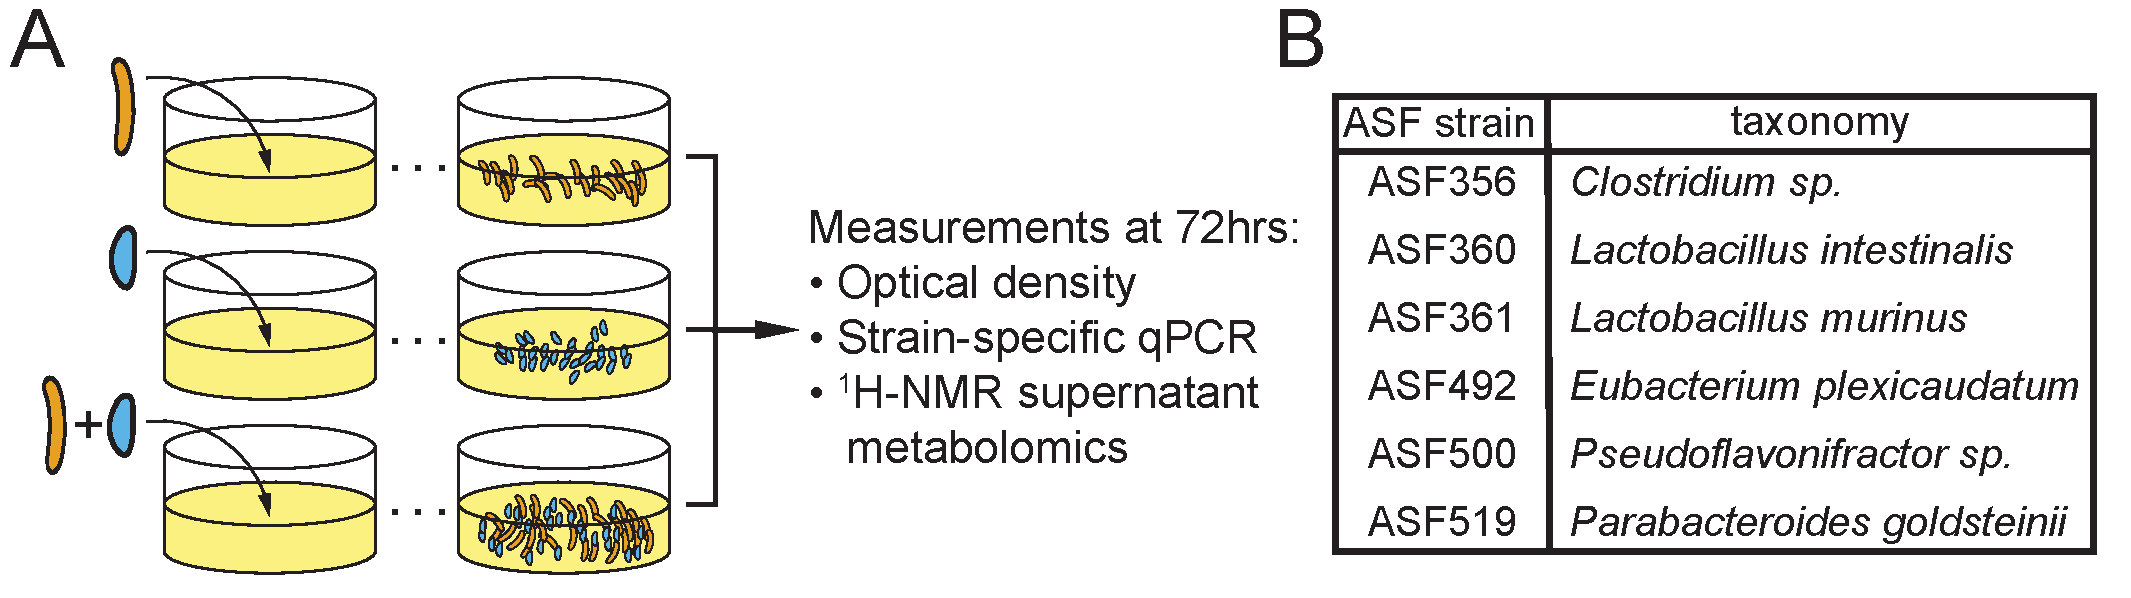
\includegraphics[width=0.8\textwidth]{ch2_fig1.tif}
\caption[Summary of co-culture experiment design, measurements, and total growth outcomes in monocultures and co-cultures.]{\textbf{Summary of co-culture experiment design, measurements, and total growth outcomes in monocultures and co-cultures.} \textbf{A)} Experimental procedure for each pair of strains and measurements taken. \textbf{B)} Taxonomic assignment for strains included in this study.}
\end{figure*}

\section{Discussion}

Text from paper

\section{Conclusion}

new conclusion section

\section{Acknowledgments}

Acknowledgements

\section{References}

%\end{refsection}



\end{document}
